% !TeX root = bash.tex
\section{Recap}
\begin{frame}
\frametitle{Last time…}
\begin{columns}
    \begin{column}{0.6\textwidth}
        \begin{itemize}
            \item File operations: \tt{cat, ls, cp, mv, rm, mkdir}
            \item CLI basics: options, arguments, shortcuts
            \item Pipes: stdin/stdout, \tt{>} and \tt{>>}
        \end{itemize}
    \end{column}
    \begin{column}{0.4\textwidth}
        
\includegraphics[width=\textwidth]{bin_cat}
    \end{column}
\end{columns}
\end{frame}

\begin{frame}
\frametitle{Before we start}
\begin{itemize}
    \item Log into a shell \textbf{right now}
    \item If you don't have a shell, you might as well leave
    \item Not sure if it's a shell or not? Ask us
    \item \tt{cd tarball/04-regex/}
    \item Type commands by hand, not Ctrl+C/V
\end{itemize}
\end{frame}

\begin{frame}[fragile]
\frametitle{Conventions in slides}
\begin{itemize}
    \item \tt{\$} indicates a \textbf{bash command}.
        Do not type the \tt{\$}.
    \item \tt{\#} indicates a \textbf{comment}.
        Do not type it or anything after it.
\end{itemize}
For example, when you see:
\begin{lstlisting}[language=bash]
$ echo hello  # printf("hello\n");
\end{lstlisting}
You are going to type:
\begin{lstlisting}[language=bash]
echo hello
\end{lstlisting}
\end{frame}

\section{IV. Regex}
\begin{frame}
\frametitle{What's a regex}
\textbf{Regex}: ``regular expressions''
\newline \newline
It's a way to match a string against \textbf{patterns}.
\newline \newline
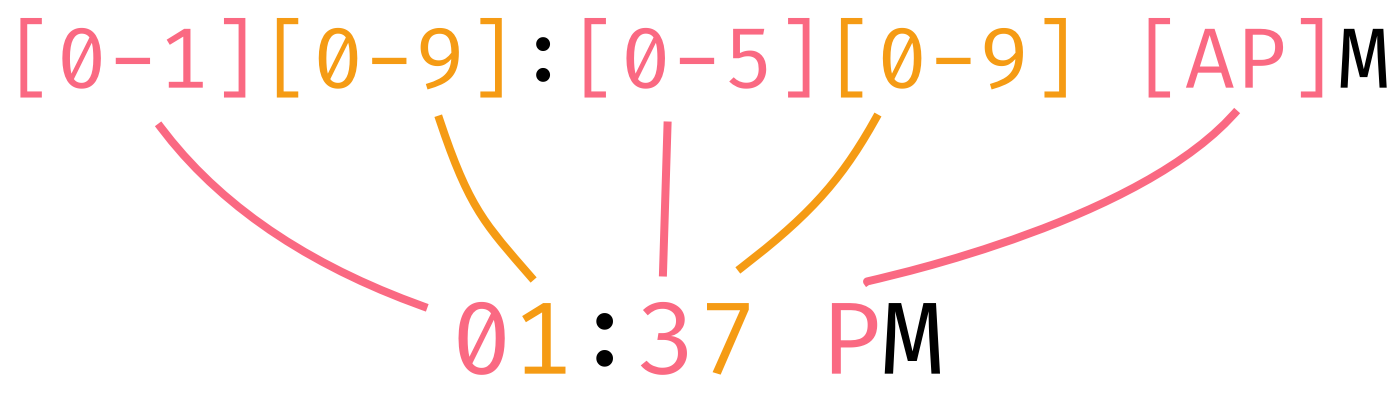
\includegraphics[width=\textwidth]{regex_breakdown}
\end{frame}

\begin{frame}[fragile]
\frametitle{Why regex?}
\begin{columns}
    \begin{column}{0.5\textwidth}
        \begin{itemize}
            \item Humans categorize things based on patterns
            \item Some patterns are really common (e.g. ``6 digit PIN'')
            \item Writing boilerplate code is slow
            \item Do not reinvent the wheel
        \end{itemize}
    \end{column}
    \begin{column}{0.5\textwidth}
        \begin{example}
            Find lines beginning with six digits with \tt{grep}:
\begin{lstlisting}[language=bash]
$ grep -E '^[0-9]{6}' file
\end{lstlisting}
            Same function, written in Python:
\begin{lstlisting}[language=python]
with open("file") as f:
  for line in f:
    if line[:6].isdigit():
      print(line.strip())
\end{lstlisting}
        \end{example}
    \end{column}
\end{columns}
\end{frame}

\begin{frame}[fragile]
\frametitle{Regex patterns: \tt{.}}
The dot is the simplest pattern:
\begin{table}
    \centering
    \begin{tabular}{ll}
        \textbf{Pattern}    & \textbf{Matches} \\
        \verb|.|            & any character \\
    \end{tabular}
\end{table}

\begin{example}
    \verb|c.t| matches \tt{cat}, \tt{cut}, \tt{c t}, and even \tt{c\$t}.
\end{example}

\begin{block}{Note}
    To match a literal dot, escape it like this: \verb|\.|
\end{block}
\end{frame}

\begin{frame}[fragile]
\frametitle{Regex patterns: \tt{[]}}
Brackets match any of the characters inside.
If \verb|^| is the first character, it means ``not''.
\begin{table}
    \centering
    \begin{tabular}{ll}
        \verb|[aeiou]|      & a vowel \\
        \verb|[^aeiou]|     & anything but a vowel \\
    \end{tabular}
\end{table}
If \verb|^| is inside \tt{[]} but not the first character, then it has no
special effect:
\begin{table}
    \centering
    \begin{tabular}{ll}
        \verb|[aeiou^]|     & not a vowel, not \verb|^| \\
        \verb|[^-^]|        & not \verb|-|, not \verb|^| \\
    \end{tabular}
\end{table}
\end{frame}

\begin{frame}[fragile]
\frametitle{Regex patterns: \tt{[]}}
If \tt{-} is between two characters, it means any character between them
(Usually in ASCII). 
\begin{table}
    \centering
    \begin{tabular}{ll}
        \verb|[0-9]|        & any digit \\
        \verb|[A-Za-z]|     & any letter \\
        \verb|[A-Za-z-]|    & any letter or \tt{-} \\
        \verb|[A-Z a-z]|    & any letter or space \\
    \end{tabular}
\end{table}
\begin{block}{Note}
    \verb|[A-z]| is \textbf{not} equivalent to \verb|[A-Za-z]| because that's
    not how ASCII works. Therefore this feature is mostly used within \tt{A-Z},
    \tt{a-z} and \tt{0-9} separately.
\end{block}
\end{frame}

\begin{frame}[fragile]
\frametitle{Regex patterns: \tt{[]}}
\verb|^| and \verb|-| can be used together:
\begin{table}
    \centering
    \begin{tabular}{ll}
        \verb|[^0-9]|           & anything but numbers \\
        \verb|[^A-Za-z]|        & anything but letters \\
        \verb|[^a-z0-9äöüß]|    & what Elon Musk will literally name his child \\
    \end{tabular}
\end{table}
Multiple instances of \verb|[]| work like cartesian products.
For example, \verb|[01][0-9]| matches \tt{00} up to \tt{19}.
\end{frame}

\begin{frame}[fragile]
\frametitle{Quiz: Does it match?}
What does \Large \verb|[um]jicanvas.com| \normalsize match?
\begin{itemize}
    \item \tt{umjicanvas.com}
    \item \tt{jicanvas.com} % neither
\end{itemize}
\pause
\begin{block}{Challenge}
    How to fix this regex? % (um)?jicanvas\.com
\end{block}
\end{frame}

\begin{frame}[fragile]
\frametitle{Regex patterns: character classes}
\begin{table}
    \centering
    \begin{tabular}{ll}
        \verb|\w|           & letters, numbers, and underscore:
                              \verb|[A-Za-z0-9_]| \\
        \verb|\W|           & anything \verb|\w| does not match \\
        \verb|\s|           & whitespace (space, tab, linebreak, etc) \\
        \verb|\S|           & anything but whitespace \\
    \end{tabular}
\end{table}

\begin{block}{Note}
    Character classes in brackets like \verb|[\w\s]| won't work.
\end{block}
\end{frame}

\begin{frame}[fragile]
\frametitle{Regex patterns: \tt{( | )}}
\tt{()} can be used to group patterns.
\tt{|} separates patterns inside \tt{()}, and matches one of them.
\begin{table}
    \centering
    \begin{tabular}{ll}
        \verb!cat|dog!              & cat or dog \\
        \verb![bc]at|[dh]og!        & bat, cat, dog, or hog \\
        \verb!(ls|cd|rm -r) dir!    & \tt{ls dir}, \tt{cd dir}, or \tt{rm -r dir} \\
    \end{tabular}
\end{table}
\end{frame}

\begin{frame}[fragile]
\frametitle{Regex patterns: repeat}
If you have a pattern that repeats, these will help:
\begin{table}
    \centering
    \begin{tabular}{ll}
        \verb|A?|           & zero or one A \\
        \verb|A+|           & one or more A's \\  % Positive closure
        \verb|A*|           & zero or more A's \\ % Kleene closure
        \verb|A{2}|         & AA \\
        \verb|A{2,4}|       & AA, AAA, or AAAA \\
        \verb|A{20,}|       & AAAAAAAAAAAAAAAAAAAA… \\
    \end{tabular}
\end{table}

\begin{example}
    \verb|C[-+]?| matches C-, C, or C+\footnote{My VV156 grade}.
\end{example}
\end{frame}

\begin{frame}[fragile]
\frametitle{Regex patterns: location}
These do not match literal characters. Instead, they specify the location of
the character before/after it.
\begin{table}
    \centering
    \begin{tabular}{ll}
        \verb|^|            & beginning of line \\
        \verb|$|            & end of line \\
        \verb|\b|           & word boundary \\
        \verb|\B|           & not word boundary \\
    \end{tabular}
\end{table}

\begin{example}
    \begin{itemize}
        \item \verb|^$| matches an empty string only
        \item \verb|\bwork\B| matches \tt{bash workshop} and \tt{worker},
            but not \tt{homework}
    \end{itemize}
\end{example}
\end{frame}

\begin{frame}[fragile]
\frametitle{Quiz: Does it match?}
What strings does this regex match? \newline

\Large \verb!(^cat)|(cat$)! \normalsize

\begin{itemize}
    \item \verb|cat|                      % yes
    \item \verb|^cat$|                    % no
    \item \verb|cats|                     % yes
    \item \verb|cat /etc/fstab|           % yes
    \item \verb|I have a cat.|            % no
    \item \verb|Cats are the best.|       % no
    \item \verb|Concatenate these files|  % no
\end{itemize}
\end{frame}

\begin{frame}[fragile]
\frametitle{grep recap}
Try this in \tt{04-regex/}:
\begin{lstlisting}[language=bash]
# Usage: grep [OPTION] PATTERN [FILE]
$ grep 'charlem' faculty
\end{lstlisting}
\begin{block}{Note}
    \begin{itemize}
        \item For Mac users, you might have to type \tt{ggrep}.
        \item Because of the countless symbols that will soon follow,
            it is advised to always wrap the pattern in quotes.
        \item If you forget \tt{FILE}, and get stuck, just press Ctrl+C.
    \end{itemize}
\end{block}
\end{frame}

\begin{frame}[fragile]
\frametitle{But how to use a regex, anyway?}
Try this in \tt{04-regex/}:
\begin{lstlisting}[language=bash]
$ grep -E '^[a-z]+\.[a-z]+@' faculty
\end{lstlisting}
\pause
\begin{block}{Observation}
    The regex matches all email addresses in the file \tt{faculty}
    that look like ``firstname.lastname@sjtu.edu.cn''.
    \newline \newline
    \tt{-E} enables regex.
\end{block}
\end{frame}

\begin{frame}[fragile]
\frametitle{One more example}
Type this in \tt{04-regex/}.
\begin{lstlisting}[language=bash]
$ grep -oE '^[^@]{,8}' faculty
\end{lstlisting}
Before you hit enter, guess: what does this regex do?
\pause
\begin{block}{Observation}
    Everything after ``@'' is gone, and each line is at most 8 characters long.
\end{block}
\begin{block}{Explanation}
    \begin{tabular}{ll}
        \verb|-o|   & Only keep the part that matches regex \\
        \verb|^|    & From beginning of each line \\
        \verb|[^@]| & Keep any character except @ \\
        \verb|{,8}| & Match 8 characters max \\
    \end{tabular}
\end{block}
\end{frame}

\begin{frame}[fragile]
\frametitle{Your turn}
Extract all course codes from \tt{04-regex/courses}. \newline

\begin{example}
    \begin{tabular}{lcl}
        VG100 Introduction to Engineering & & VG100 \\
        VM020 Machineshop Training & $\Longrightarrow$ & VM020 \\
        VP140 Physics I & & VP140
    \end{tabular}
\end{example}
\pause
\begin{block}{Solution}
\begin{lstlisting}[language=bash]
$ grep -oE 'V[A-Z][0-9]{3}' courses
\end{lstlisting}
\end{block}
\end{frame}

\begin{frame}[fragile]
\frametitle{Find and replace with \tt{sed}}
\tt{sed} is a powerful tool for transforming text. However, I have only
used one very specific syntax for substitution:
\footnote{
    When the pattern/replacement contains slashes, you can use things like
    \tt{!} and \tt{,} as delimiters.
}
\begin{lstlisting}[language=bash]
$ sed -E 's/FIND/REPLACE/FLAGS' [FILE]
\end{lstlisting}
\begin{block}{Note}
    \begin{itemize}
        \item For Mac users, use \tt{gsed}
        \item Again, \tt{-E} enables regex
        \item \tt{FIND} is a regex
        \item \tt{FLAGS} is optional
        \item If \tt{FILE} is not given, sed will read from stdin
    \end{itemize}
\end{block}
\end{frame}

\begin{frame}[fragile]
\frametitle{Find and replace with \tt{sed}}
This command redacts all the IPv4 addresses in the file \tt{ipv4}:
\begin{lstlisting}[language=bash]
$ sed -E 's/([0-9]+\.){3}[0-9]+/redacted/g' ipv4
\end{lstlisting}
\begin{block}{Observe}
    What will happen without the \tt{g} at the end?
\end{block}
\end{frame}

\begin{frame}[fragile]
\frametitle{Capturing groups}
What if you \textbf{don't} want to replace something?
\bigskip

When you put a pattern inside \tt{()}, it becomes a \textbf{capturing group},
or simply \textbf{group}.
The content are available via \textbf{backreferences} which look like
\verb|\1|, \verb|\2|, up to \verb|\9|.
\end{frame}

\begin{frame}[fragile]
\frametitle{Capturing groups}
When nested, the position of `\verb|(|' determines order, so the outside group
is \verb|\1| and the inside is \verb|\2|.
\bigskip

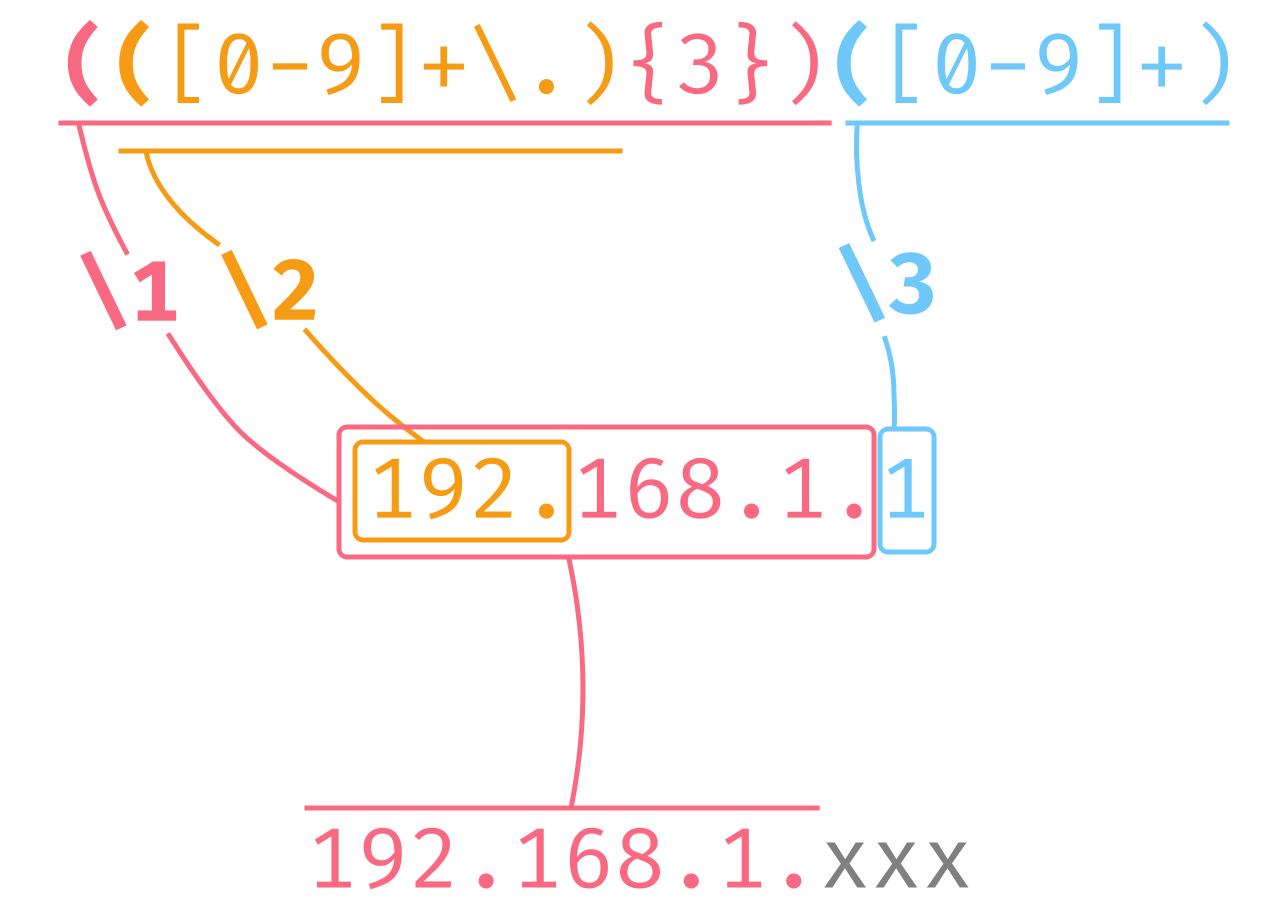
\includegraphics[width=0.8\textwidth]{capgroup_breakdown}
\end{frame}

\begin{frame}[fragile]
\frametitle{Capturing groups with \tt{sed}}
What if you only want to redact the subnet (i.e. last part) of the IP addresses?
\begin{lstlisting}[language=bash]
$ sed -E 's/(([0-9]+\.){3})[0-9]+/\1xxx/g' ipv4
\end{lstlisting}
\begin{block}{Observation}
    IP addresses like \tt{192.168.1.1} become \tt{192.168.1.xxx}
\end{block}
\end{frame}

\begin{frame}[fragile]
\frametitle{Challenge}
From \tt{04-regex/courses}, select 100- and 200-level math courses and convert
legacy ``VV'' course codes into modern ``MATH'' codes.
Do not print other courses.
\begin{example}
    \begin{tabular}{lcl}
        VV156 & & MATH1560J \\
        VV214 & $\Longrightarrow$ & MATH2140J \\
        VV417 & & \textit{not printed}
    \end{tabular}
\end{example}
\pause
\begin{block}{Hint}
    \begin{itemize}
        \item What two operations are we doing?
        \item Is \tt{sed} enough?
        \item What do we capture?
    \end{itemize}
\end{block}
\end{frame}

\begin{frame}[fragile]
\frametitle{Solution}
Two solutions are both correct:
\begin{lstlisting}[language=bash]
# 1. grep, then sed
$ grep -E 'VV[12]' courses | \
    sed -E 's/VV([0-9]{3})/MATH\10J/'

# 2. sed, then grep
$ sed -E 's/VV([0-9]{3})/MATH\10J/' | \
    grep -E 'MATH[12]'
\end{lstlisting}
\begin{block}{Note}
    \begin{itemize}
        \item \verb|\| means ``continue on next line''.
        \item \verb|\10| does not mean group 10! It means group 1, followed by
            a 0.
    \end{itemize}
\end{block}
\end{frame}

\begin{frame}
\frametitle{When not to use regex?}
\begin{columns}
    \begin{column}{0.7\textwidth}
        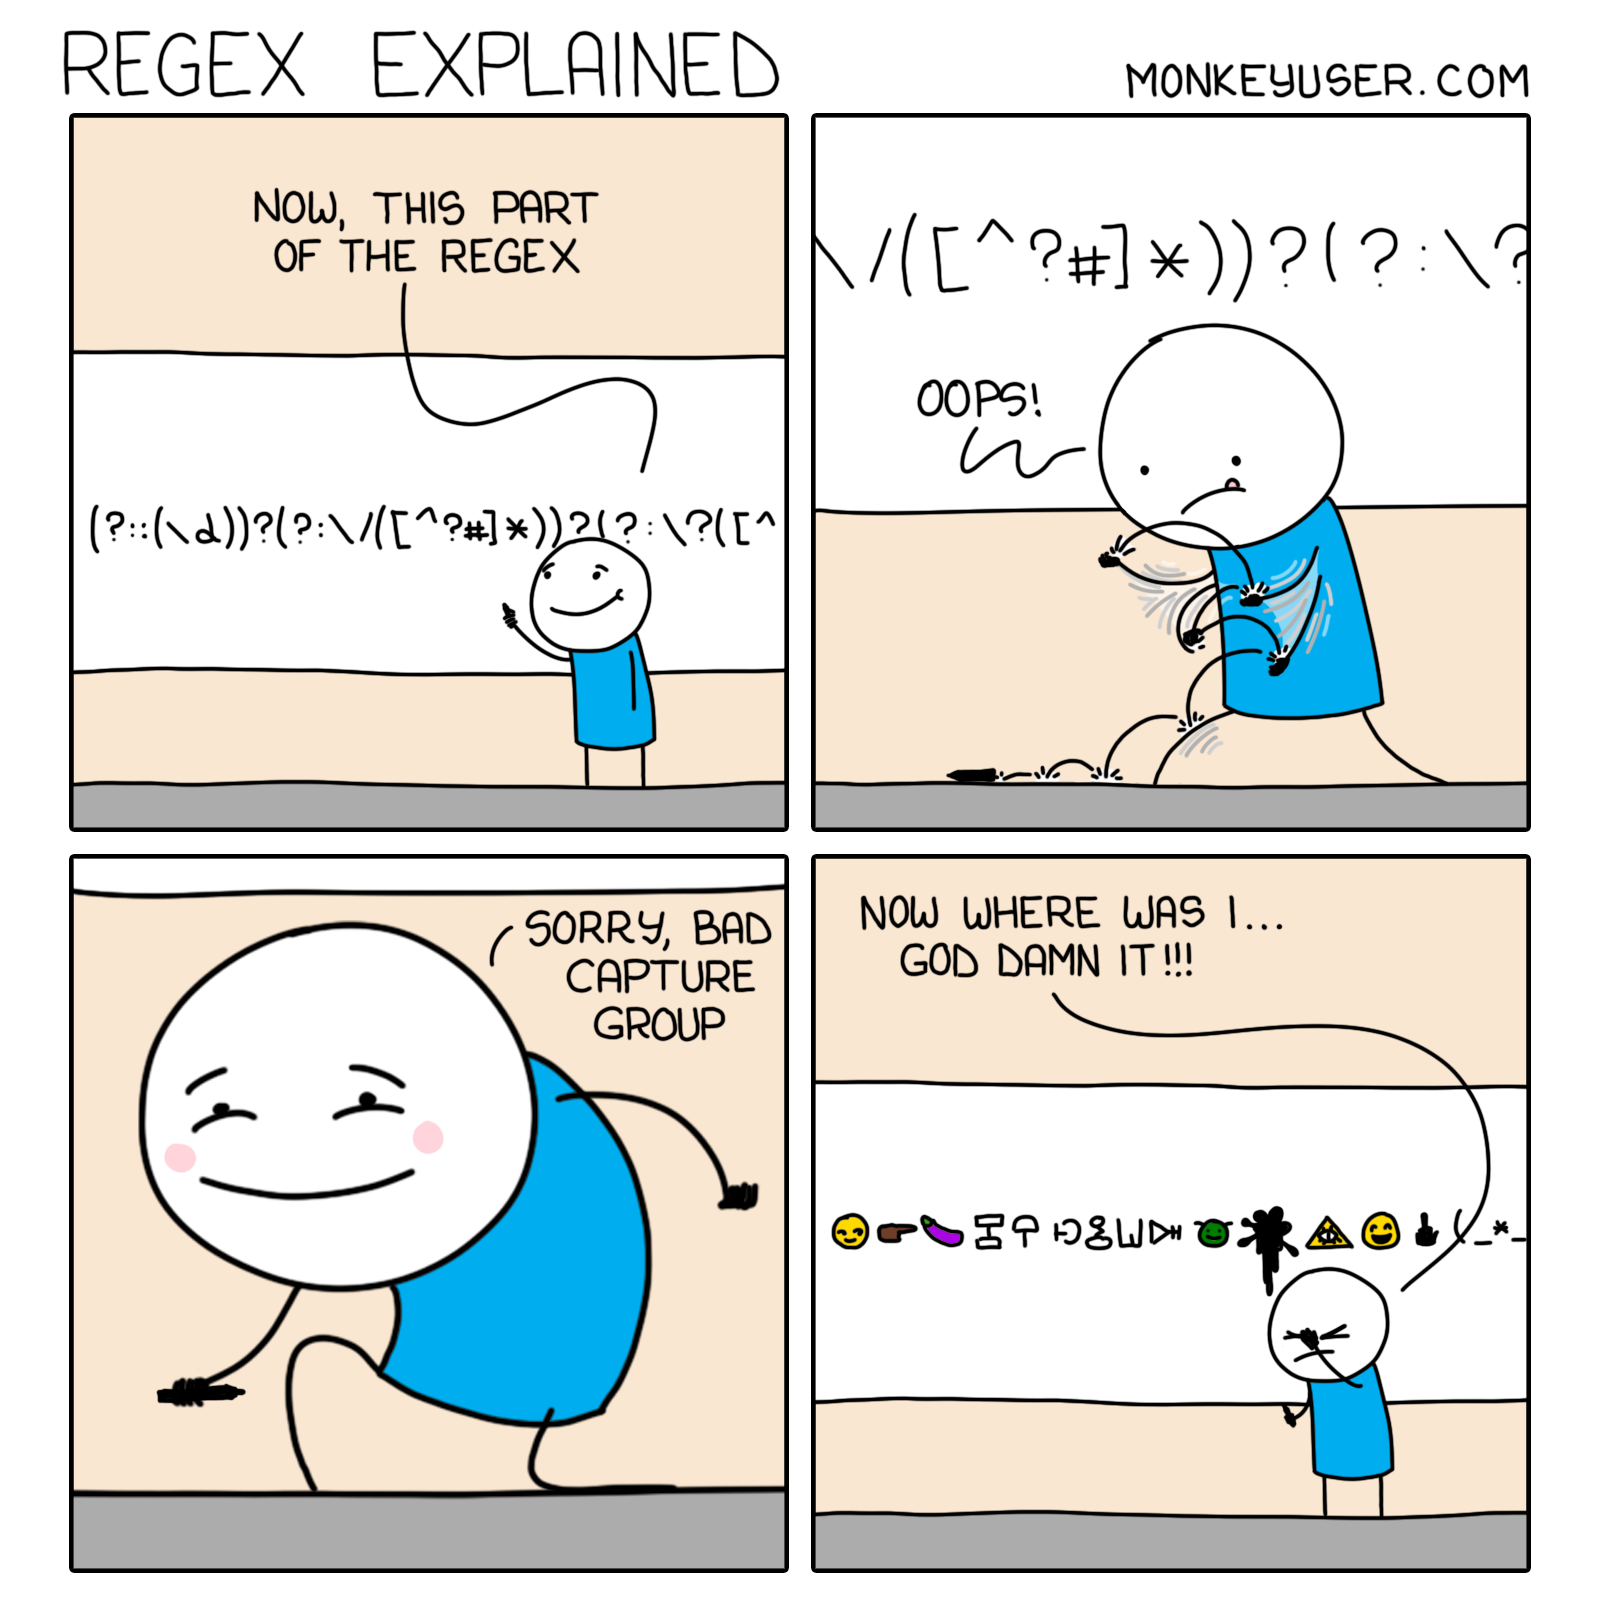
\includegraphics[width=\textwidth]{regex_explained}
    \end{column}
    \begin{column}{0.3\textwidth}
        If your regex:
        \begin{itemize}
            \item is 50 characters long
            \item handles lots of non-ASCII
            \item has too many backslashes
        \end{itemize}
        consider something else.
    \end{column}
\end{columns}
\end{frame}

\begin{frame}[fragile]
\frametitle{Atrocities under regex's name}
If you match a Chinese resident ID with \verb|[0-9]{18}|, people whose
ID ends with X will be mad at you.
\bigskip

Apart from ignorance, people also abuse regex for fun. This is a regex
that matches a JavaScript regex:
\begin{lstlisting}
/\/((?![*+?])(?:[^\r\n\[/\\]|\\.|\[(?:[^\r\n\]\\]|\\.)*\])+)\/((?:g(?:im?|mi?)?|i(?:gm?|mg?)?|m(?:gi?|ig?)?)?)/
\end{lstlisting}

And here's one that matches integers that are divisible by 3:
\begin{lstlisting}
^(?:[0369] |
(?:[147](?:[147][0369]*[258]|[0369])*[258]) |
(?:[258](?:[258][0369]*[147]|[0369])*[147]))+$
\end{lstlisting}

(These two examples are not ERE.)
\end{frame}

\begin{frame}
\frametitle{Regex is a mess}
\begin{block}{Quote}
I define UNIX as 30 definitions of regular expressions living under one roof.
\begin{flushright}
    — Donald Knuth\footnote{Digital Typography, ch. 33, p. 649 (1999)}
\end{flushright}
\end{block}

Two dominant standards:
\begin{itemize}
    \item \textbf{ERE} (Extended RegEx, used in most CLI tools)
    \item \textbf{PCRE} (Perl Compatible RegEx, used in Perl and Python)
\end{itemize}
What we talked about today is ERE.
\end{frame}
\begin{frame}
\frametitle{Beyond the workshop}
Regex101 (\url{https://regex101.com/}) is an online regular expression
evaluator that supports ERE, PCRE, and many others.
\end{frame}
